\documentclass[../pheader.tex]{subfiles}

\begin{document}
{\sc Ayudantía 2 - EDO\hfill \small\rm Apuntes: Sebastián Sánchez}

\begin{center}
    \begin{tabular}{rl}
        Docente:& Nikola Kamburov\\
        Ayudante:& Jorge Acuña
    \end{tabular}
\end{center}

% P1
\begin{problema}
Sea \(f\in C^1(\mathbb{R})\) y \(a\in \mathbb{R}\) un punto de equilibrio de la
ecuación \(\dot{x} = f(x)\). Demuestre que \(a\) es estable si \(f'(a) < 0\).

Bajo las mismas condiciones, demuestre que existen constantes positivas
\(\alpha, \delta, C\) tales que si \(\abs{x_0 - a} < \delta\) entonces
\(\abs{x(t;x_0) - a} < C\cdot e^{-\alpha t} \abs{x_0 - a}\).
\end{problema}
% R1
\begin{proof}
Sea \(\delta > 0\) y tomemos \(x \in \left(a-\delta, a+\delta\right)\). Luego,
\[
    f(x) = f(a) + f'(a) (a-x) + \phi(x)
\]
donde \(\phi(x)\) es la función de error. Como \(a\) es un punto de
equilibrio, \(f(a) = 0\). Además, \(f'(a) \ne 0\), así que el término \(\phi(x)\)
es despreciable, quedándonos
\[
    f(x) \approx f'(a) (a-x)
\]
Así, como \(f'(a) < 0\), \(f(x)\) decrece exponencialmente cuando \(x < a\) y
crece exponencialmente cuando \(x > a\).

Sabemos que \(f'(a) < 0\) y continua, así que existe un \(\delta > 0\) tal que
para \(\abs{x_0 - a} < \delta\) entonces \(f'(x_0) < 0\), en particular,
\(\max_{x\in \left(a-\delta,a+\delta\right)} f'(x) < 0\). Como en \(a\) la
función \(f\) se anula, debemos analizar el caso derecho e izquierdo por
separado (y en realidad son análogos).

Comencemos con \(x \in \left(a-\delta,a\right) = I\). Luego, \(f(x) \ne 0\) y por lo
tanto tenemos la igualdad
\[
    \int_{x_0}^{x} \frac{du}{f(u)} = t - t_0
.\]
Por TVM, existe \(\xi \in I\) tal que
\[
    \frac{f(a)-f(x)}{a-x} = f'(\xi) < \max_{I} f'
    \implies
    f(x) > \underbrace{f(a)}_{=0} + \max_{I} f' \cdot (a-x)
\]
y por lo tanto
\[
    t - t_0
    =
    \int_{x_0}^{x} \frac{du}{f(u)}
    <
    \int_{x_0}^{x} \frac{du}{(a-u) \max_{I} f'}
    =
    \frac{1}{\max_{I} f'} \int_{x_0}^{x} \frac{du}{a-u}
    =
    \frac{1}{\max_{I} f'} \log\left(\frac{a-x_0}{a-x}\right)
\]
de lo que despejando se obtiene que
\[
    \left(a - x\right) < \left(a-x_0\right)
    \exp\left(
        -\left(t - t_0\right) \max_{I} f'
    \right)
\]
Tomando \(\alpha = \max_{I} f'\) y \(C = \exp\left(t_0
\alpha\right)\) nos queda la desigualdad buscada
\[
    \left(a - x\right) < C \left(a-x_0\right) e^{-\alpha t}
.\]
El caso por la derecha es análogo y con eso obtenemos el valor absoluto.
\end{proof}

% P2
\begin{problema}
Sea
\[
    g(y) \coloneqq
    \begin{cases}
        \left(y^2 - 1\right)^2 y^3 \sin\left(y^{-1}\right)
            &, y\in \mathbb{R}\setminus \left\{ 0 \right\} \\
        0 &, y = 0
    \end{cases}
.\]
Encuentre los puntos de equilibrio de la ecuación \(\dot{y} = g(y)\) y
clasifíquelos.
\end{problema}
% R2
\begin{proof}
La función \(g(y)\) se anula en \(y = 0, \pm 1, 1/(k\pi)\). Veamos la derivada
en cada uno de estos puntos. Derivando obtenemos
\[
    g'(y) = \left[4y^2(y^2-1) + 3y^2 (y^2-1)^2\right]\sin\left(y^{-1}\right)
    + y^3 (y^2-1)^2 \cos\left(y^{-1}\right)
.\]
De esta forma \(g'(\pm 1) = g'(0) = 0\), así que debemos analizar estos casos
más en detalle. Para \(k\) par, \(g'(1/k\pi) < 0\) así que es estable, por otro
lado, si \(k\) es impar, \(g'(1/k\pi) > 0\) y el punto es inestable.

Ahora veamos los casos especiales. En todos lo casos consideramos \(h\) un real
positivo pequeño.
\begin{clist}
\item Para \(y=0\), notemos que \(g(y-h) > 0\) y \(g(y+h) > 0\). Como no hay un cambio
de signo y \(g(0) = 0\), el punto es semiestable.

\item Para \(y=1\), notemos que \(g(y-h) > 0\) y \(g(y+h) > 0\) y por lo tanto el
punto es semistable.

\item Para \(y=-1\), \(g(y-h) > 0\) y \(g(y+h) > 0\) y como antes concluimos que
el punto es semiestable.
\end{clist}
\end{proof}

% P3
\begin{problema}
Describa cómo cambia el retrato de fase correspondiente a la ecuación dada
cuando varía el parámetro \(r\in \mathbb{R}\), i.e dibuje el diagrama de
bifurcaciones. Clasifique las bifurcaciones que ocurren y calcule el(los)
valor(es) de bifurcación de \(r\):
{\setlength\multicolsep{0pt}
\begin{multicols}{2}
\begin{enumerate}[topsep=0pt,itemsep=0pt]
    \item \(\dot{x} = r - 3x^2\).
    \item \(\dot{x} = 5 - re^{-x^2}\).
    \item \(\dot{x} = x - rx(1-x)\).
    \item \(\dot{x} = rx - 4x^3\).
\end{enumerate}
\end{multicols}}
\end{problema}
% R3
\begin{proof}[Solución]
\(\dot{x} = r - 3x^2\).\\
Podemos observar que la bifurcación es de tipo silla/nodo pues la curva
\(y = r\) y \(y=3x^2\) pasan de tener \(0\) a dos puntos intersecciones. Veamos
los casos específicos.
\begin{clist}
    \item Para \(r = 0\) hay un punto de equilibrio y es semiestable.
    \item Para \(r > 0\) hay dos puntos \(x_1*\) y \(x_2*\) de equilibrio.
    El primero es inestable y el segundo es estable.
    \item Para \(r < 0\) no hay puntos de equilibrio.
\end{clist}

\noindent\rule{\linewidth}{.1pt}
\(\dot{x} = 5 - re^{-x^2}\).\\
La curva que tenemos es \(r =
5e^{x^2}\). Luego, \(5e^{x^2} \ge 5\) y forma dos curvas simétricas con respecto
al eje \(r\). De esta forma,
\begin{clist}
\item Si \(r < 5\) entonces no hay puntos de equilibrio.
\item Si \(r = 5\) hay un solo punto y es semiestable (en sentido negativo), pues a la
derecha e izquierda del punto la curva \(5e^{x^2}\) está sobre la recta \(r=5\).
\item Si \(r > 5\) hay dos puntos de equilibrio. Para \(x* < 0\) el punto es
inestable y para \(x* > 0\) estable.
\end{clist}
La bifuración es de tipo silla/nodo.

\noindent\rule{\linewidth}{.1pt}
\(\dot{x} = x - rx(1-x) = f(x,r)\).\\
La curva de nivel da \(x = rx(1-x)\), es
decir, es el conjunto \(\left\{x = 0\right\} \cup \left\{r = \frac{1}{1-x}\right\}\).

Para este caso, lo mejor es pensar en los puntos de equilibrio como la
intersección entre la curva \(y = x\) y \(y = rx(1-x)\). La última es una
parábola con ceros \(x= 0\) y \(x=1\) y la concavidad depende el \(r\). Además,
la intersección de la parábola con la recta se da cuando
\[
    x = rx(1-x) = rx - rx^2
    \iff
    rx^2 + (1-r)x = 0
    \implies
    x = \frac{-(1-r) \pm \abs{1-r}}{2r}
\]
notar que si \(r = 1\) entonces \(x = 0\) es la única intersección.
\sideToSide{.45}%
{%
    \begin{figure}[H]
    \caption{Gráfico de la curva de nivel \(f(x,y) = 0\).}
    \centering
    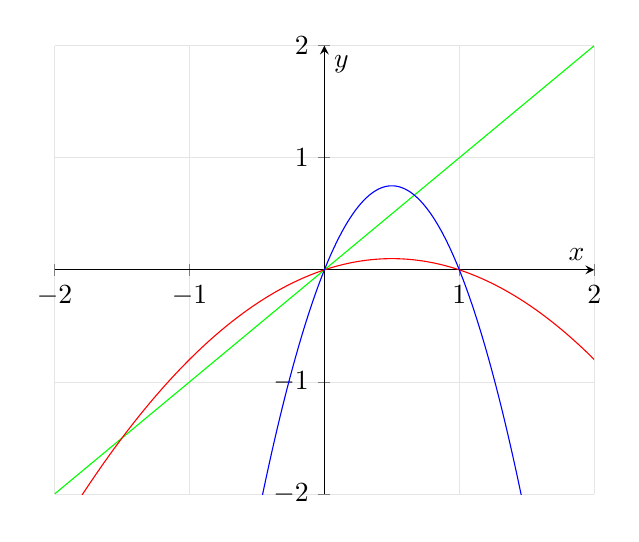
\begin{tikzpicture}
    \def\r{.5};
    \begin{axis}[
        grid=both,
        grid style={very thin, gray!20!white},
        axis lines = middle,
        xlabel = {\(x\)},
        ylabel = {\(y\)},
        xmin=-2, xmax=2,
        ymin=-2, ymax=2]

    \addplot[green] coordinates {(-2,-2)(2,2)};

    \addplot[red, samples=500] {0.4*x*(1-x)};
    \addplot[blue,samples=500] {3*x*(1-x)};
    \end{axis}
    \end{tikzpicture}
    \end{figure}
}%
{%
\begin{clist}
    \item Si \(r=0\) la parábola colapsa a una recta y al única intersección es
    en \(x = 0\). Luego, \(x=0\) es un punto intestable pues para \(x < 0\) se
    tiene que \(f(x,r) < 0\) y para \(x > 0\) se tiene que \(f(x,r) > 0\).

    \item Si \(r=1\) tenemos una sola intersección en \(x=0\). El punto es
    -- dado que \(f(x,r) > 0\) si \(x < 0\) y \(f(x,r) < 0\)
\end{clist}
}%

\noindent\rule{\linewidth}{.1pt}
\(\dot{x} = rx - 4x^3\).
\end{proof}

% P4
\begin{problema}
La velocidad \(v(t)\) en una caída libre se puede modelar por
\[
    m\dot{v} = mg - kv^2
\]
donde \(m\) es la masa del objeto, \(g\) es la aceleración de gravedad y \(k >
0\) es una constante relacionada con la resistencia del aire.
\begin{itemize}[itemsep=0pt]
    \item Encuentre los puntos de equilibrio y clasifíquelos.
    \item Calcule \(\lim_{t\to\infty} v(t)\) (conocidad como velocidad
    terminal).
\end{itemize}
\end{problema}
% R4
\begin{proof}
\begin{itemize}
    \item Veamos la curva de nivel \(f(v,m,g,k) = g - \frac{k}{m} v^2 = 0\),
    esto nos deja \(g = \frac{k}{m}v^2\). Dado que \(g > 0\) y \(k/m > 0\) hay dos
    puntos de equilibrio, pues la recta \(y=m\) intersecta dos veces a la parábola \(y
    = \frac{k}{m}v^2\).

    Llamemos \(v_1 < v_2\) a los puntos de equilibrio.

    A la izquierda de \(v_1\) la parábola está sobre la recta, así que \(f <
    0\). Por la derecha de \(v_1\) la parábola está bajo la recta, así que \(f >
    0\). Concluimos entonces que \(v_1\) es inestable.

    A la izquierda de \(v_2\) la parábola está bajo la recta, así que \(f > 0\),
    mientras que para valores a la derecha de \(v_2\) la recta está arriba de la
    parábola, así que \(f < 0\). Concluimos que \(v_2\) es estable.

    \item
\end{itemize}
\end{proof}
\end{document}
